\section{Prostheses}
\paragraph{Stump prosthesis}
Following an amputation, there is often a functional need for a prosthesis.
Traditionally, these contain a socket wherein the residual limb (stump) is placed, hence their name.
The reduced loads experienced by the skeleton lead to loss of bone density; and, particularly for leg prostheses, friction against the socket, uneven loads on the soft tissue, and other abuses cause severe and sometimes chronic skin problems \citep{levy_skin_1980} --- to the point that some may refuse to wear their prosthetics.

\paragraph{ITAP}
Intraosseous transcutaneous amputation prostheses (ITAP) \cite{kang_osseocutaneous_2010} are bone-anchored, skin-crossing devices which provide amputees an alternative attachment of artificial limbs, bypassing the role of the residual limb's soft tissue (See Figure \ref{fig:ITAP}).
The purpose of ITAP is to transfer the loads from the skeleton directly to the artificial limb, while simultaneously achieving cutaneous integration, i.e. avoiding infection and other problems associated with breaking the skin barrier.

\begin{figure}\centering
    \begin{subfigure}{0.45\textwidth}\centering
        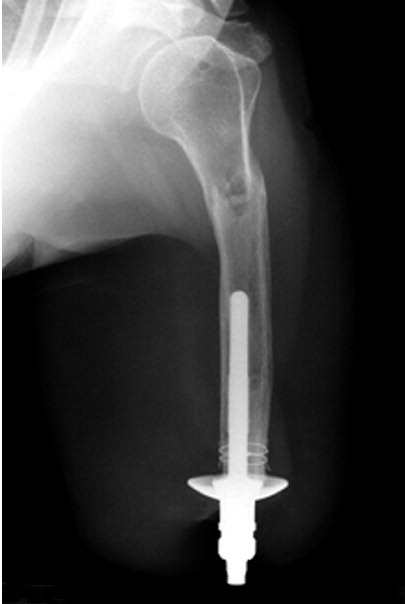
\includegraphics[height = 7cm]{figures/ITAP-xray.jpg}
        \caption{Adapted with permission from Kang et al \cite{kang_osseocutaneous_2010}.}
    \end{subfigure}
    \begin{subfigure}{0.45\textwidth}\centering
        {\small \incfig[0.67]{ITAP-scheme}}
        \caption{}
    \end{subfigure}
    \caption{X-ray of ITAP inserted into femur (a) and ITAP anatomy (b). Note how ITAP bypasses the load-bearing role of traditional stump prostheses, allowing loads to be transferred from the skeleton through the ITAP onto the artificial limb,}
    \label{fig:ITAP}
\end{figure}

\section{Vibrotactile (haptic) feedback}
An amputation is not just the loss of a limb, but also the loss of tactile feedback, a fundamental way we gather information about the world around us.
Generally, prosthetics users rely on visual feedback and secondary cues, such as sound or changes in pressure on the residual limb \cite{schofield_applications_2014}, suggesting at best an indirect level of proprioception.
Sensory feedback, particularly through the use of vibrations (i.e. vibrotactile), is associated with better object recognition, manipulation and grip force control \cite{schiefer_artificial_2018, rosenbaum-chou_development_2016}.
For stump prostheses, sensory feedback must be achieved through electrical stimulation of soft tissue.
We hypothesise that bones' ability to perceive vibrations in so-called osseoperception \cite{OrgelMarcus2021Oito}, combined with ITAP, can be the vehicle for haptic feedback.

In order to overcome both limitations of vibration motors and a patient's ability to resolve discrete frequencies, there is motivation to use both frequency and particular vibration patterns, e.g. ascending amplitudes, pauses between vibrations, etc.   
We see reasonable success in people's ability to distinguish vibration patterns \cite{ChaubeyPravin2014Cvhf}, and even bypass some of the traditional challenges of mounting vibration motors on skin by placing them on the ITAP. 
For low-frequency stimulations on soft tissue, patients are able to distinguish between 1 Hz and 2 Hz with an accuracy of 71\% \cite{ChaubeyPravin2014Cvhf}, while in the range of \SIrange{60}{360}{Hz} patients have been shown to be able to distinguish 6 levels of vibration \cite{rosenbaum-chou_development_2016}.
Because we ultimately focus on osseoperception, the frequency range of about \SIrange{1}{350}{Hz} will simply serve as guidance as to what is clinically relevant.

\section{Project goals}
Depending on the bone quality of the residuum, ITAP may be press-fitted or cemented into the remaining bone in the amputated limb.
It is unclear what effect this has on vibrations propagating through ITAP that are transmitted to the bone and surrounding soft tissue.
This projects creates the foundations to answer this question, and it aims to \textbf{characterise vibrations propagating through ITAP}.
Ultimately we are trying to understand \begin{enumerate}
    \item How vibrations propagate through ITAP
    \item How can we control the amplitude of vibrations?
\end{enumerate}

These results feed into a larger research project that, in the short tern, ensures the safety and reliability of haptic feedback, and in long term sees its use in the development of sophisticated cognitive control over artificial limbs.

\section{Methods}
This project investigates the propagation of vibrations along an ITAP device by generating a computer aided design (CAD) model (Abaqus, Dassault Systemes).
It uses a modal analysis to help inform the appropriate frequency range, then applies a concentrated point-force on the spigot prescribing a linear displacement according to equation \ref{eq:sin-eq}, where $\textbf{s}$ is displacement in mm, $t$ is time, $f$ is linear frequency, $z$ is a Cartesian axis.
It explores the effects of each of the following parameters as they pertain to the periodic force input: frequency, amplitude, duration and position.
Both modal analysis and prescribed linear displacement are carried out using Abaqus/Standard.


\begin{equation} \label{eq:sin-eq}
    \textbf{s}_z(t) = 0.2\sin(2\pi f t)
\end{equation}


\subsection{CAD Model}
A model ITAP is designed with stem length of \SI{120}{mm} and a proximal stem radius of \SI{6}{mm}, narrowing to \SI{4.5}{mm} distally.
The collar has a height of \SI{6}{mm} mm and radius of \SI{14}{mm}.
The spigot has a height of \SI{45}{mm} and radius of \SI{9}{mm}.

The CAD model has a \SI{2.5}{mm}, hexahedral-dominated mesh (element types C3D8R and C3D6) with 4300 elements and properties that of Titanium 6--4, i.e., elastic material of density \SI{4430}{\kilo\gram\per\metre\cubed}, Young's modulus \SI{114}{\giga\pascal} and Poisson's ratio 0.33.

% phase aims to determine the effect on vibrations of each of the following: the presence of the flange, different stem diameters, and the presence of bone cement.
% It begins with a simple metal rod and builds up to an ITAP such that it is possible to parametise both its characteristics and the interface with bone.
% Finally, it will ascertain whether there is a measurable difference between the forces at the ITAP-bone interface for cemented and press-fitted implants.

% \begin{figure}[h]\centering
%     \begin{tikzpicture}[scale=0.85]
%         \begin{axis}[
%             xlabel = ITAP length, ylabel = Amplitude, title = Generate waves and define damping ratio,
%             domain=0:40,xtick=\empty, ytick=\empty,
%             samples=100,
%             axis lines = left, ymax=1.2, ymin=-1.2
%             ]
%             \addplot[] {cos(deg(x))*exp(-0.1*x)};
%             \addplot[dashed] {exp(-0.1*x)};
%             \legend{Generated wave, Damping ratio}
%         \end{axis}
% \end{tikzpicture}
% \begin{tikzpicture}[scale=0.85]
%     \begin{axis}[
%         xlabel = ITAP length, ylabel = Amplitude, title = Experimentally determine threshold of perception,
%         domain=0:40,
%         samples=100,xtick=\empty, ytick=\empty,
%         axis lines = left, ymax=1.2, ymin=-1.2,
%         align=center,
%         ]
%         \addplot[] {cos(deg(x))*exp(-0.1*x)};
%         \addplot[dashed, red, domain=30:40] {0.02};
%         % \draw[-stealth] (axis cs: 35,0.5) node[above]{Perception \\ Threshold}-- (axis cs: 35,0.05);
%         \addplot[dashed] coordinates {(30,-0.8) (30,0.3)};
%         \draw (axis cs: 30,-0.8) node[below]{ITAP-Tissue interface};
%         \legend{Generated wave, Perception Threshold}
%     \end{axis}
% \end{tikzpicture}
% \caption{The experimental procedure has two phases: Defining the damping ratio along the ITAP, and determining the threshold for perception.}
% \label{fig:model-data}
% \end{figure}

% The subsequent protoyping phase aims to establish a threshold of perception for soft tissue and to validate the computational model.
% This phase will progress similarly, beginning with the metal rod design and finishing with an ITAP of one particular dimension; emulating the ITAP-bone and ITAP-soft tissue interfaces.